  \documentclass[12pt]{article}
    \usepackage{amsmath}
    \usepackage{graphicx}
    \usepackage{multirow}
    \usepackage{booktabs}
    \usepackage{subfigure}
    \usepackage{verbatim}
    \usepackage{color}
    \usepackage{hyperref}
    \usepackage{url}
    \usepackage{axessibility} 
    
    
    \begin{document}

    \title{PHYS131 -- IT Skills -- Worksheet 5 -- A report on High-Temperature Superconductors }
    \author{Samuel Hedges}
    \date{\today}
    \maketitle

    \begin{abstract}
     \textit{A paper on the development of Superconductivity from its discovery by \cite{Onnes} in 1911 from cooling mercury with liquid helium to the 2020 discovery of room temperature superconductors \cite{Room-Temperature Superconductivity}} and how they may be useful in future technologies \cite{Lancaster}.
    \end{abstract}

    \tableofcontents
\section{Introduction To Superconductivity}


A superconductor is defined as the sudden disappearance of all electrical resistance when cooled below a certain temperature known as the \textit{critical temperature} \cite{Y&F}. A high-temperature superconductor is a superconductor which has a critical temperature above 77 Kelvin, denoted K, (the boiling point of liquid nitrogen) \cite{2}.\\

\section{Brief History and Theory of Superconductors}

Superconductivity was first observed by Heike Kamerlingh Onnes in 1911. He was studying the resistance of solid mercury at cryogenic temperature using the then recently developed Liquid Hydrogen as a coolant. At the temperature of 4.2 K he observed the resistance of abruptly disappear \cite{Onnes}. Great strides would be made in the understanding of superconductors, Meissner and Ochsenfield would observe superconductors expelling magnetic fields \cite{Meissner Effect}. This phenomenon, now known as the Meissner Effect would later be described by Fritz and Heinz London's Equations known as the London equations in 1935:

\begin{equation}
\frac{\partial\mathbf{j}}{\partial t} = \frac{n_{s}e^2}{m}E   
\end{equation}

\begin{equation}
 \nabla \times \textbf{j} = \frac{n_{s}e^2}{m}B   
\end{equation} 

Where: $\mathbf{j}$ is the current density, $E$ the magnetic field, $B$ the magnetic field, \textit{e} the charge of the electron, \textit{m} the mass of the electron and $n_{s}$ is a constant \cite{London Equations}\\

These Laws were derived from Ohms Law: The current is proportional to the electric field; The Lorentz Force Law: 

\begin{equation}
F = qE + qv \times B
\end{equation}

and Faraday's Law:

\begin{equation}
-\frac{\partial B}{\partial t} = \nabla \times E
\end{equation}

These equations describe why the resistance drops to zero when the temperature drops below the critical temperature although this is a classical explanation.  
\\
In 1987 the first high-temperature superconductor that could be cooled by liquid nitrogen, and not Helium, was found. a yttrium-based cuprate perovskite material \cite{93 K Superconductor}. This discovery would open up superconductors for use in more technologies as liquid nitrogen is easier to produce than liquid helium and mitigated risk involved in pressure buildups that resulted from the use of liquid helium. \\
 

\section{The First Room Temperature Superconductor}
\label{sec:PDU}
In October of last year the first Room-temperature superconductor was observed by a team headed by Professor Ranga Dias at the University of Rochester \cite{NYT}. This team was able to get a superconductivity at 287 K (roughly 15 Degrees Celsius) in a carbonaceous sulphur hydride. This Superconductivity occurred at 267$ \pm {10} Gigapascals$ \cite{Room-Temperature Superconductivity}.
\\

\begin{figure}[!ht]
    \centering
    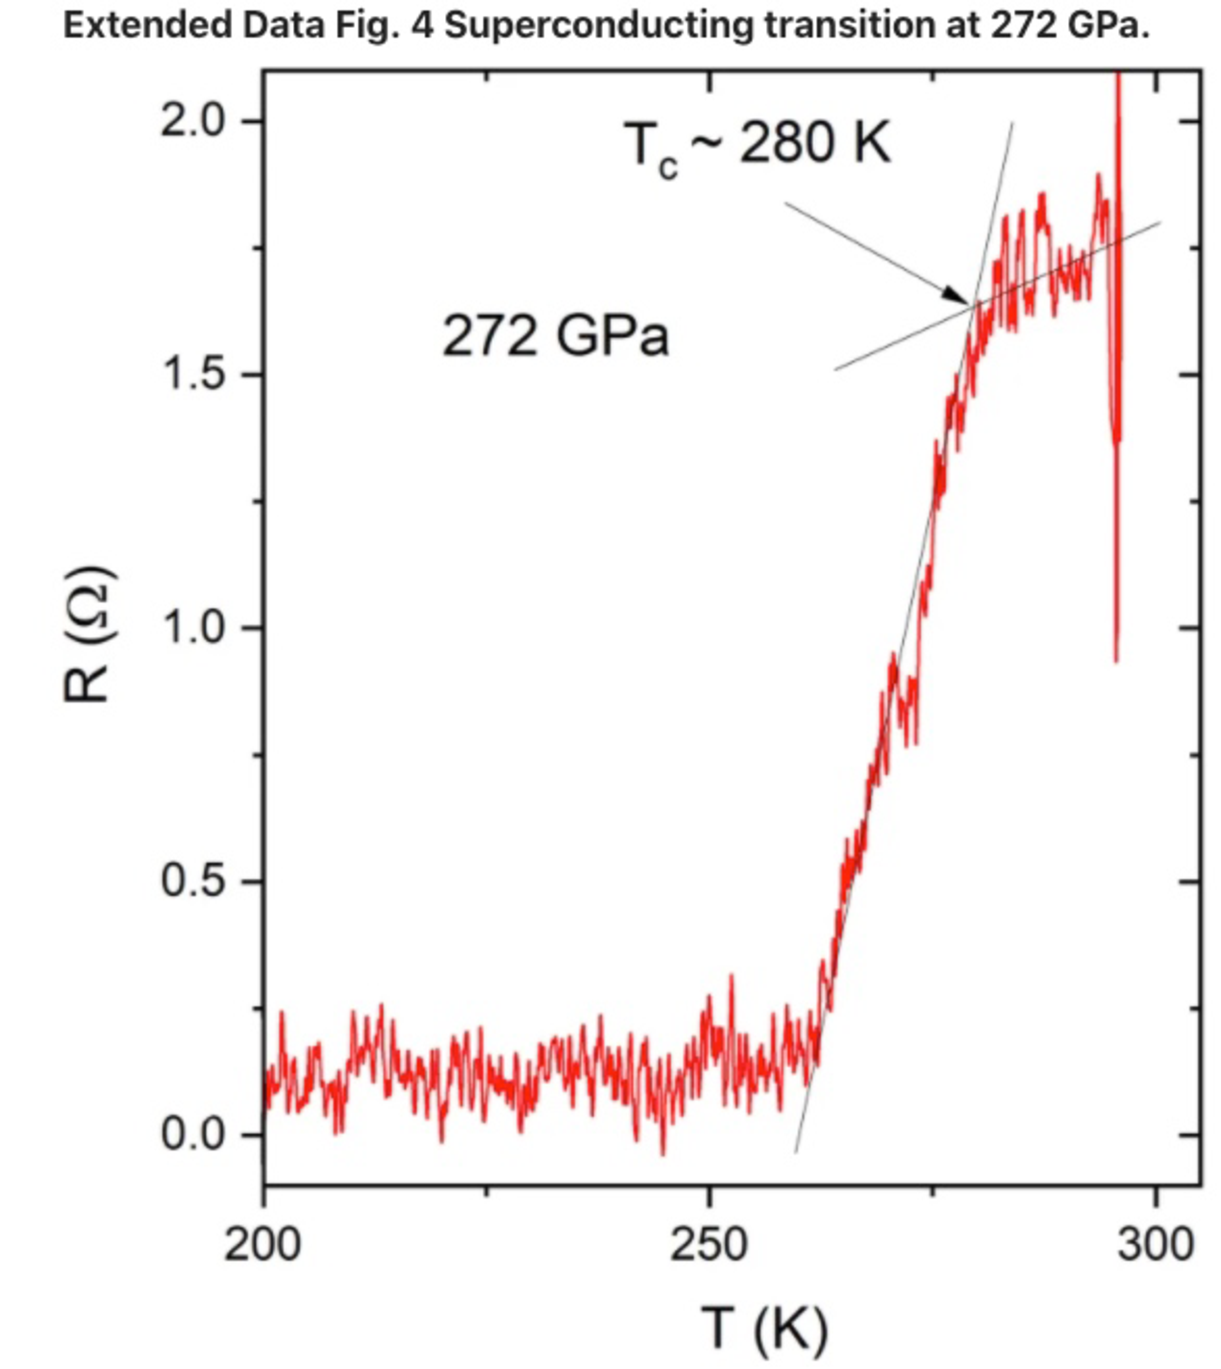
\includegraphics[scale=0.5]{Week 5 - Research Paper/Tue, 16 Feb 2021, 14_43.pdf}
    \caption{The Illustration Published in the journal nature showing  carbonaceous sulphur hydride Superconducting at 280 K and 272 GPa \cite{Room-Temperature Superconductivity}} 
    \label{fig:my_label}
\end{figure}


\section{Summary}

\begin{center}
    \begin{figure}[!ht]
    \begin{tabular}{|c|c|c|}
    \hline
\multirow{2}{*}{High-Temperature Superconductors} & 287 Kelvin &  carbonaceous sulphur hydride \\ 

& 93 Kelvin & yttrium-based cuprate perovskite\\ \hline

\color{white} \colorbox{blue}{Coolant} & \color{white} \colorbox{blue}{77 Kelvin} & \color{white} \colorbox{blue}{Liquid Nitrogen Boiling Point} \\ \hline

\multirow{2}{*}{Type I Superconductor} & 7 Kelvin & Lead\\ 
& 4.2 Kelvin & Mercury\\\hline 

\color{white} \colorbox{blue}{Coolant} & \color{white} \colorbox{blue}{4 Kelvin} & \color{white} \colorbox{blue}{Liquid Helium Boiling Point}\\\hline

    \end{tabular}
    \caption{A table of the Temperature of the coolants and superconductors With lower temperatures at the bottom and higher temperatures at the top}
    \end{figure}
\end{center}
 As is summarised in the table above, the many superconductors found at higher temperatures than ever with  the 2020 discovery \cite{Room-Temperature Superconductivity} leading to new research being undertaken to find a superconductor than can work at higher temperatures and atmosphere lower pressures. An example in the field is The work underway at Lancaster University where a collaborative team are using superconductors to try and create microwave single photon sources and detectors.\cite{Lancaster}

\begin{thebibliography}{99}
\bibitem{Y&F}‘Sears and Zemansky’s University Physics with Modern Physics Fifteenth Edition in SI Units’, Hugh
D. Young and Roger A. Freedman, Pearson Education (2020)
\bibitem{2} Timmer, John (May 2011). "25 years on, the search for higher-temp superconductors continues". Ars Technica.
\bibitem{Onnes} Kamerlingh Onnes, Heike (1911) "Further experiments with liquid helium. C. On the change of electric resistance of pure metals at very low temperatures etc. IV. The resistance of pure mercury at helium temperatures"
\bibitem{Meissner Effect} W. Meissner and R. Ochsenfeld (1933). "Ein neuer Effekt bei Eintritt der Supraleitfähigkeit". Naturwissenschaften. 21 (44): 787–788
\bibitem{London Equations} London, F,;London, H. (1935). "The Electromagnetic Equations of Superconductor" \textit{Proceedings of teh Royal Society A: Mathematics, Physical and Engineering Sciences}
\bibitem{93 K Superconductor} M. K. WU; et al (1987) "Superconductivity at 93 K in a New Mixed-Phase Y-Ba-Cu-O Compound System at Ambient Pressure" \textit{Physical Review Letters} \textbf{58} 
\bibitem{NYT} A Warmer Superconductor, Kenneth Chang, The New York Time October 27th 2020, Section D, Page 3
\bibitem{Room-Temperature Superconductivity} Snidet, E., Dasenbrock-Gammon., R. et al. Room-temperature superconductivity in carbonaceous sulfur hydride. Nature 586, 373-377 (2020).
\bibitem{Lancaster} Superconducting Quantum Circuits,https://www.lancaster.ac.uk/quantum-technology/research/superconducting-quantum-circuits/,Professor Yuri Pashkin and  Dr Jonathan Prance
\end{thebibliography}


    \end{document}
